\section{Previous works}
In the past, a number of previous works been made about this topic. While the participation of mobile devices to the Grid was theorized, it was never concretized (especially due to technical limitations). This section presents three previous works that provide interesting concept and ideas that influence the solution offered by this work.

\subsection{Proxy-Based Cluster Architecture (2002)}
In early 2000s, \textit{Thomas Phan}, \textit{Lloyd Huang} and \textit{Chris Dulan} proposed a solution to integrate devices with low capabilities (such as PDAa) into Grid computing. The work is highly influenced by the technical difficulties resulting from the technological panorama at the time, trying to \textbf{isolate the new devices in a sub-environment that can be integrated into the Grid without affecting its inner workings}.

\subsubsection{Architecture}
\begin{figure}[H]
    \centering
    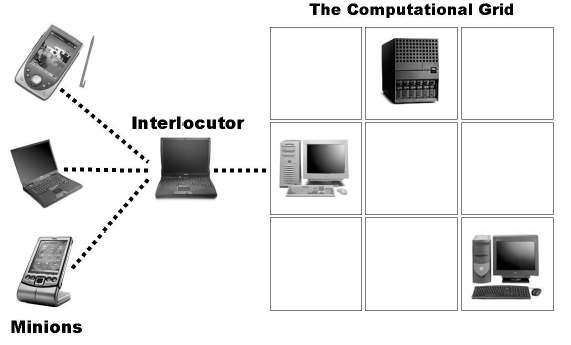
\includegraphics[scale=0.9]{document/chapters/chapter_3/images/2002_architecture.png}
    \caption{Proxy-Based Cluster Architecture \cite{integrating_mobile_devices_into_grid}}
    \label{fig:2002_architecture}
\end{figure}
This architecture revolves around the idea of having a \textbf{cluster} constituted by a number of \textbf{BASELINE} (Barely Adequate Systems Leveraging Internet NEtworking) \textbf{devices} that act as \textbf{\textit{Minions}}. Such BASELINE devices coexist (in the \textbf{same wireless network}) with a \textbf{proxy device} powerful enough to coordinate them. In this architecture, this proxy device is known as \textbf{\textit{Interlocutor}}; this machine runs a software that acts as a middleware with an existing Grid system.

\begin{quotation}
    \textit{"When a resource request arrives at the Interlocutor from a resource consumer, the request is handled by the Interlocutor. For simplicity, we proceed in this example with the assumption that the request is for CPU time to process incoming data. The interlocutor must decompose the request accordingly among its minions; [...]. After the problem has been distributed to the minions, the interlocutor waits for results and sends them back to the requester. The Interlocutor has the option of aggregating the data before responding with the result in order to amortize the cost of per-message communication overhead." \cite{integrating_mobile_devices_into_grid}}
\end{quotation}

\subsubsection{Interesting concepts and ideas}
One of the strengths of such architecture is \textbf{delegation}; Minions rely entirely on the Interlocutor, taking only the active decision (based on the user's will) to either participate or not to the Grid. Having such division in responsibilities \textbf{simplifies the software running on BASELINE devices} (which was the one mostly affected by compatibility issues given the number of OSes for PDAs) while moving such complexity on the stabler and more standardized Interlocutor.
Another advantage gained from this architecture is the \textbf{reduction of latency}. Since the devices operate under the same wireless network, a requestor that is located anywhere on the planet has only to execute a long request to the Interlocutor, while coordination in the cluster is almost instantaneous given the short distances.
The local coordination allows \textbf{managing resources more easily} since the responsibility of determinate whether certain resources are available and/or adequate becomes distributed between all Interlocutors.
\textbf{Device discovery is also greatly simplified} since the Grid services do not actually need to discover every single BASELINE device but only Interlocutors.
Furthermore, \textbf{the Interlocutor hides devices heterogeneity from the Grid}, allowing also to possibility to apply mechanisms to compensate for BASELINE devices performances.

While using a local Interlocutor seems very effective, every benefit gained by the use of it comes at the cost of a great limitation: \textbf{when it comes to practically scaling the Grid, having the devices operating under the same local network makes extremely more difficult for volunteers to offer their devices}. It is still possible to use some sort of variation of an Interlocutor, but this obviously comes at the cost of loosing some benefits such the reduction of latency while operating in the same network.

\subsection{Mobile-to-Grid Middleware (2005)}
While the previous work focused on mobile devices contributing to the Grid, this one (by \textit{Umar Kalim}, \textit{Hassan Jameel}, \textit{Ali Sajjad} and \textit{Sungyoung Lee}) provides a solution for \textbf{enabling the possibility for mobile devices to utilize the Grid's services}.
The \textbf{Middleware gateway} represents the main element in this architecture, allowing mobile devices (running a client) to access Grid's services through it; using this expedient, limitations on computational power needed on requestor's devices are eliminated, making possible to \textbf{trigger complex operations even from a device that is not adequate in performances}.

\subsubsection{Architecture}
A machine devolved to act as a Middleware gateway runs three different modules:
\begin{itemize}
    \item \textbf{Middleware service}\\
    The main software module that handles access to Grid's resources by the clients executing requested operations.
    \item \textbf{Ontology server}\\
    Used to gain access to information that define different possible client devices.
    \item \textbf{UDDI registry}\\
    The discovery of Middleware gateways by mobile devices is performing by using the UDDI registry where every new instance of the gateways is registered. Hence, a machine acting as a Middleware gateway needs this module to interact with such registry.
\end{itemize}

\begin{figure}[H]
    \centering
    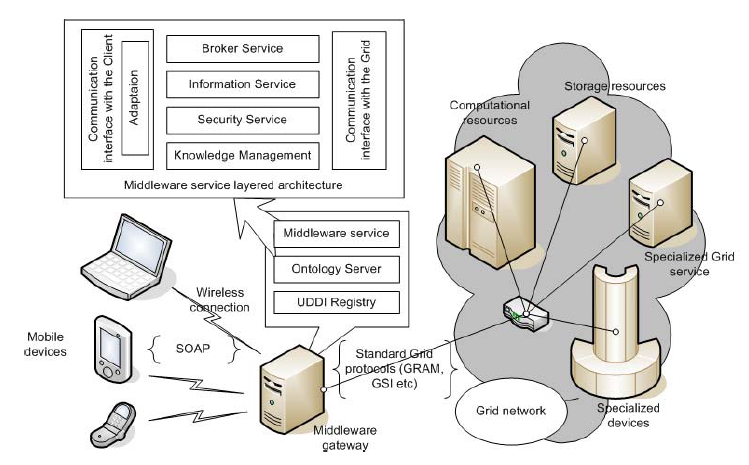
\includegraphics[scale=0.8]{document/chapters/chapter_3/images/2005_architecture.png}
    \caption{Mobile-to-Grid Middleware \cite{mobile_to_grid_middleware}}
    \label{fig:2005_architecture}
\end{figure}
\vspace{10mm}

\begin{quotation}
    \textit{"Firstly the client application discovers and connects with the Middleware. Then the service, after authentication, submits its device specification along with the job request. The middleware then locates the relevant Grid service and after authorization forwards the request. The client may then request some status information (regarding the job or the service). If the client wishes to disconnect (and collect the result later), the Middleware would facilitate a soft state registration and to which would later help in the reintegration. After disconnection all the requests are served locally (with the cached information). Requests that result in updates at the Middleware service are logged for execution at reconnection. Upon reconnection pending instructions are executed and information updates at the client end are made to maintain consistency." \cite{mobile_to_grid_middleware}}
\end{quotation}

The Middleware service, being the most complex module among the three, is built with a service layered architecture:
\begin{itemize}
    \item \textbf{Broker service}\\
    This service takes job requests from the Client devices and, after verifying that adequate Grid's services are available (using the Information service), downloads the code to be executed (from the device or from another source) and start to perform the job interacting with the Grid. Results are stored in the Knowledge management layer.
    \item \textbf{Knowledge management}\\
    This layer manages relevant information, both on the client side and on the Grid side. Here results are also scaled down and/or formatted before being returned to the Client device.
    \item \textbf{Security service}\\
    Here there are all the security measures used to create a safe and authenticated connection with both the mobile Client and the Grid. 
    \item \textbf{Information service}\\
    With this service determinate which services and resources are available on the Grid.
    \item \textbf{Communication interface with the Grid}\\
    This layer handles the implementation of communication protocols established by the Grid.
    \item \textbf{Communication interface with the Client}\\
    Similarly, this layer has the responsibility to perform communication with the Client running on a device; given the different types of possible clients running on different devices, an Adaption module is added to implement device-specific communication (using information gained by the Ontology server)
\end{itemize}

\subsubsection{Interesting concepts and ideas}
The main advantage of this idea is the \textbf{versatility obtained by increasing the number of devices capable of using the Grid's services}. Development on the requestor side is greatly simplified, removing heterogeneity since the actual complexity is moved to the Middleware gateway. To extend compatibility of devices, it is just necessary to implement the communication modules on the new client and add a new Adaption module in the Middleware service.

While this is surely a great advantage, \textbf{it comes at a great price: the necessity to provide machines that act as a Middleware gateway}. Considering that the computation is mainly done in such machines (with the collaboration of the peers inside the Grid), this results in an intense usage, \textbf{increasing costs for the Grid owners}.
As the paper also states, there is also a \textbf{problem with scalability}. If a client submits a task and disconnects from the gateway (whether voluntarily of involuntarily), there is no guarantee that it will later reconnect to the same Middleware gateway, requiring mechanisms to deal with this issue.

\subsection{Autonomous Mobile Middleware (2006)}
TODO

\subsubsection{Architecture}
TODO

\subsubsection{Protocols}
TODO

\subsubsection{API examples}
TODO

\subsubsection{Interesting concepts and ideas}
TODO